\documentclass[a4paper,12pt]{scrreprt}                       % default is A4 paper style and 11pt font size


%%%%%%%%%%%% version history %%%%%%%%%%%%%%%%%%%%%%%%%%%%%%%%%%%

%26.03.2017:    corrections for the latex source-code: diacritics issues; corrected the glossaries and added listings packages; added fontspec (only works with xelatex/lualatex !!!)
%2014:          put in latex version + some small additions - Florin Stoican
%2013:          content from Dan Stefanoiu
%%%%%%%%%%%%%%%%%%%%%%%%%%%%%%%%%%%%%%%%%%%%%%%%%%%%%%%%%%%%%%%%%%%%%%%%%


%%%%%%%%%%%% macros for various paths %%%%%%%%%%%%%%%%%%%%%%%%%%%%%%%%%%%
\def \cls {./cls} 																					 % path to common latex files (change for your own relative/absolute path)
\def \pics {./pics}      																		 % path to pics files (change for your own relative/absolute path)
\def \chapters {./chapters}      														 % path to chapter files (change for your own relative/absolute path)
\def \code {./code}      													        	 % path to source code files (change for your own relative/absolute path)

% you don't have to use them but it's nicer this way
%%%%%%%%%%%%%%%%%%%%%%%%%%%%%%%%%%%%%%%%%%%%%%%%%%%%%%%%%%%%%%%%%%%%%%%%%
\usepackage{tikz}
\usepackage{pgfplots}
\usepackage{float}
\usepackage{svg}
\newcommand{\norm}[1]{\left\lVert#1\right\rVert}
\usepackage[parfill]{parskip}
%\usepackage{subfig}
% language={english/romanian} selects between the languages used in the manusript (changes, e.g., the name of the chapter)
% type={bachelor/master/phd} selects between the type of manusript (changes, e.g., the titlepage make-up)
\usepackage[language=romanian,type=bachelor]{\cls/standard} % introduces useful packages and commands(CHANGE ONLY IF YOU KNOW WHAT YOU'RE DOING)
\addbibresource{\cls/bib.bib}																% bib resource (using biblatex package, for complex stuff use the biber backend instead of bibtex
\newglossaryentry{computer}
{
  name=computer,
  description={is a programmable machine that receives input,
               stores and manipulates data, and provides
               output in a useful format}
}

\newacronym[longplural={Frames per Second}]{fpsLabel}{FPS}{Frame per Second}
\newacronym{lvm}{LVM}{Logical Volume Manager}        																	% put here all your glossary terms; only the ones actually used will appear in the glossary list of the manuscript

\begin{document}

%%%%%%%%%%%%%%%%%%%%%%% frontmatter %%%%%%%%%%%%%%%%%%%%%%%%%%%%%%%%%%%%%
\pagenumbering{roman}																				% default numbering for the frontmatter is roman

\title{Clasificare defecte într-o rețea de apă de mari dimensiuni}														% title of your manuscript
\author{Cazan Cristian-Claudiu}																				% author name
\advisor{Florin Stoican}																			% advisor name

\maketitle

% show table of contents, figures, tables and algorithms

\tableofcontents 
\printnoidxglossaries																				% \printglossaries works only if the makeindex has the correct arguments
\addcontentsline{toc}{chapter}{\listfigurename}
\listoffigures 
\addcontentsline{toc}{chapter}{\listtablename}
\listoftables
\addcontentsline{toc}{chapter}{\listalgorithmcfname}
\listofalgorithmes

\clearpage

%%%%%%%%%%%%%%%%%%%%%%% mainmatter %%%%%%%%%%%%%%%%%%%%%%%%%%%%%%%%%%%%%%
\pagenumbering{arabic}																			% default numbering for the mainmatter is arabic

% here is the text of you manuscript; you can put it directly here but it is better to include files (the main file will be more compact)
\chapter{Introducere}
\label{chap:intro}

\section{Motivația alegerii temei}
Transportul și distribuția apei reprezintă una dintre cele mai vechi preocupări inginerești de proporții, existând de mai mult de 4000 de ani. Civilizația minoică, localizată în insula Creta, este considerată a fi prima care a construit apeducte - structuri pentru transportul apei de la sursă către orașe - în 2500 î.Hr. 

Deși majoritatea popoarelor din antichitate care s-au ocupat cu construcția apeductelor întrebuințau aceste sisteme pentru irigația pământului - ocupațiile de bază de atunci fiind în strânsă legătură cu agricultura - romanii au văzut în sistemele de provizionare a apei și un potențial imens în dezvoltarea civilizației, astfel ei sunt ei care aduc cele mai mari contribuții inginerești, apeductele construite de aceștia impresionând și astăzi prin grandoarea și iscusunța cu care au fost construite.

Inovațiile în acest domeniu au suferit salturi bruște și puternice în momentul descoperirii unei noi relații matematice care transformă un parametru despre care se puteau face doar niște estimări grosiere într-o mărime bine definită și bine controlată. Istoric vorbind începutul dezvoltării științei hidraulice s-a bazat pe relația descoperită de Arhimede din Siracuza în sec III î.Hr, $F = V_{obiect} \cdot \rho_{lichid}*g$. O altă contribuție care are o deosebită importanță în domeniul tehnologiei de distribuiție a apei și nu numai o reprezintă tubul lui Pitot folosit la măsurarea vitezei fluidului, inventat de Henri Pitot în sec XVII. Din punct de vedere constructiv tubul are o formă de \textbf{L}, scufundarea acestuia într-un fluid (apă sau gaz) va determina creșterea nivelului și a presiunii până la o anumită limită \cite{klopfenstein1998air}, ecuația care guvernează depedența nivel - viteză este:
\begin{equation}
u = \sqrt{\frac{2(p_t-p_s)}{\rho}} 
\end{equation}

unde:

\begin{description}
\item u reprezintă viteza fluidului;
\item $p_t$ reprezintă presiunea de stagnare;
\item $p_s$ reprezintă presiunea statică;
\item $\rho$ reprezintă densitatea fluidului.
\end{description}

Mergând mai departe, alte contribuții importante apar din partea marilor matematicieni precum Daniel Bernoulli și Leonhard Euler, care au mărit spectrul mecanicii lui Newton și Leibniz spre aria hidraulicii și a termodinamicii. Fluidele considerate sunt incompresibile și au densitatea constantă în timp și uniform distribuită în spațiu. Bernoulli afirmă despre lichidele incompresibile că o creștere în viteză a lichidului este însoțită de o scădere a energiei potențiale a lichidului (i.e. a presiunii):
\begin{equation}
\frac{u^2}{2} + gz + \frac{p}{\rho} = c
\end{equation}

unde:
\begin{description}
\item v reprezintă viteza fluidului;
\item g reprezintă accelerația la care e supus fluidul;
\item z reprezintă elevația ștrangulației conductei;
\item p reprezintă presiunea într-un anumit punct;
\item $\rho$ reprezintă densitatea fluidului.
\end{description}

În contextul în care se dorește analiza unui caz real este important ca toate diferențele între cazurile ideale și cazurile reale să fie puse în evidență în mod matematic, astfel se particularizează ecuația generală Navier-Stokes pentru cazuri în care se cunosc anumiți parametrii ai sistemului de analizat. Spre exemplu ecuația Poisuille care modelează începutul fluxului de apă într-o conductă este \cite{elger2016engineering}:
\begin{equation}
\frac{\partial u}{\partial t} = \frac{G}{\rho} + \nu \left( \frac{\partial^2 u}{\partial t^2} + \frac{1}{r}\frac{\partial u}{\partial{r}}\right)
\end{equation}

unde:
\begin{description}
\item $u$ reprezintă viteza lichidului prin conductă
\item $t$ reprezintă timpul
\item $G$ reprezintă diferența de presiune
\item $\rho$ reprezintă densitatea lichidului
\item $\nu$ reprezintă vâscozitatea cinematică
\item $r$ reprezintă poziția
\end{description}

Se poate observa că pe măsură ce modelul matematic se apropie de realitate, complexitatea acestuia crește și pentru fiecare situație specială - spre exemplu analiza presiunii la  introducerea apei într-o conductă vs. analiza presiunii când conducta este încărcată cu apă - are nevoie de o ecuație specială sau de o particularizare a ecuației Navier-Stokes, pentru care încă nu se cunoaște dacă există soluții pentru cazul cu 3 dimensiuni și dacă soluțiile acestea sunt netede. 

Ținând cont de importanța apei în desfășurarea activităților cotidiene atât pentru oameni cât și pentru actorii importanți ai industriei, este o condiție absolut necesară ca un oraș să aibă un sistem performant de distribuție a apei. În contextul actual al dezvoltării tehnologiei este natural să folosim tehnici moderne de monitorizare a diferiților parametrii din cadrul unei rețele pentru a putea face o analiză riguroasă și eficientă cu referire nu numai la mentenanță ci și la consumul global și local în ideea îmbunătățirii și reducerii pierderilor.


\section{Expunerea problemei}

În această lucrare se va aborda problematica identificării prezenței unui defect - \textit{Fault detection} și izolarea defectului \textit{Fault isolation} apărut într-un nod al rețelei - aceasta reprezentând o simplificare deoarece un defect apare de obicei într-una din conductele rețelei legate de acel nod. Combinănd cei doi termeni obținem \textit{Fauld detection and Isolation} (FDI).

O rețea de apă poate fi privită ca un graf neorientat $G = (V, E)$ unde $V$ este mulțimea nodurilor rețelei - acestea reprezentând o abstractizare asupra componentelor precum:
\begin{itemize}
\item rezervoare
\item tancuri de apă
\item puncte de distribuție
\end{itemize} 

$E$ este mulțimea muchiilor reprezentând de fapt țevile care fac legătura între noduri.

Mergând mai departe cu abstractizarea se pot considera rețele de apă active și rețele de apă pasive. Diferența între cele două făcându-se în baza pompelor de apă amplasate în zonele unde presiunea sau elevația vin în detrimentul distribuției apei.

Rețelele de apă care vor fi tratate în această lucrare fac parte din categoria pasivă, astfel putem diviza mulțimea nodurilor $V$ în $V^t$ și în $V^j$ reprezentând mulțimea nodurilor de tip tanc și mulțimea nodurilor joncțiune, cu proprietatea că $V = V^t \cup V^j$. Tancurile și rezervoarele dintr-o rețea de apă au proprietatea că nivelul de apă din acestea se va menține la un nivel oarecum staționar, astfel simulările din capitolele viitoare se vor axa pe nodurile simple de tip joncțiune, deci mulțimea de interes în acest caz va fi $V^j$ pentru care cunoaștem cardinalul.

Caracteristicile care se pot recolta dintr-o rețea de apă pot varia în funcție de elementul inspectat și de senzorii dispuși în rețea, astfel pentru fiecare nod $n_i \in V^j$ putem defini la fiecare moment de timp 
\begin{itemize}
\item presiunea $p_i(t)$ - măsurată în metri coloană de apă $mH2O$, mărime influențată puternic de presiunea interioară a nodului și de eventualele perturbații exterioare i.e. scurgeri de apă prin conducte;
\item 'cererea' $d_i(t)$ - măsurată $L/s$, mărime ce caracterizează profilul de utilizare al utilizatorilor de-a lungul unei zile i.e. debitul de apă care ajunge la consumatori. Acest debit poate varia de-a lungul zilei, putem distinge de exemplu intervale de timp în care cererea este foarte mică și rețeaua intră în regim staționar;
\item de asemenea pentru fiecare conductă a rețelei $e_{ij} \in E$ putem măsura viteza lichidului $v_{ij}(t)$.
\end{itemize}



Pentru a putea rezolva problema de FDI este importantă găsirea unei modalități eficiente de selecție și prelucrare a datelor de la rețea.Mai mult, punând în lumină aspectul ingineresc al problemei, trebuie găsită o submulțime $V_{opt} \subset V^j$ ai cărei elemente pot aduce informații necesare și suficiente pentru a detecta un defect într-o acoperire destul de mare a rețelei.

\section{Exemplul de lucru}
În următoarele capitole și în implementarea lucrării consider rețeaua Hanoi iar pentru simularea scenariilor propuse voi folosi biblioteca și suita de funcții \textbf{EPANET} - Environmental Protection Agency NETwork \cite{rossman2000epanet}. 

\noindent Rețeaua Hanoi constă într-o mulțime de noduri de tip joncțiune $V^j$ cu $|V^j| = 31$ și mulțimea $V^t$ cu $|V^t|=1$, ilustrată în figura de mai jos:
 
\begin{figure}[h]
\centering
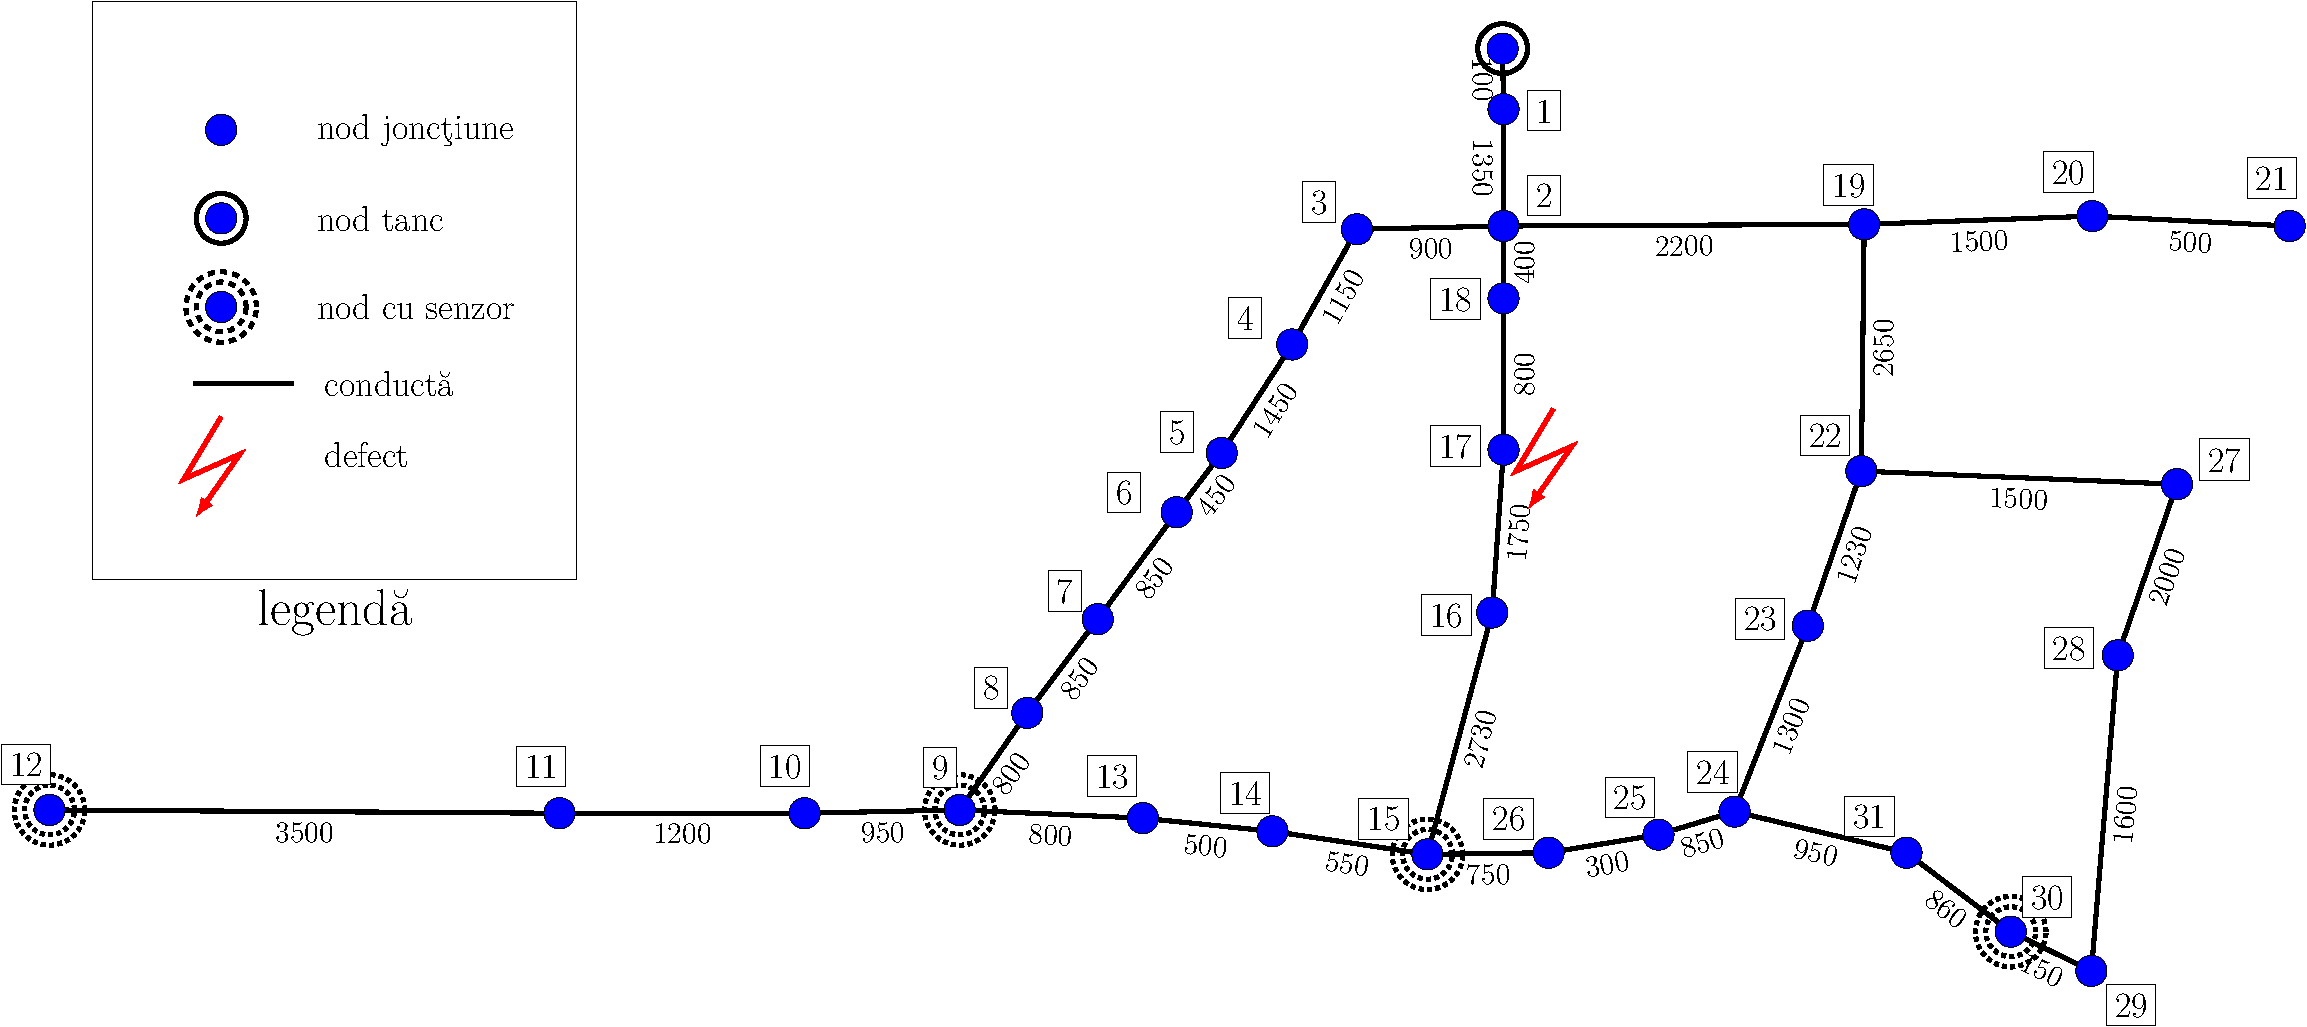
\includegraphics[width=\textwidth]{pics/c1_pics/hanoi_network.pdf}
\caption{Graful rețelei de apă din Hanoi \cite{irofti2017dictionary}}
\label{fig:hanoinetwork}
\end{figure}

După cum se poate observa în figura de mai sus au fost reprezentate două tipuri de node pasive, anume tancurile și joncțiunile. În cazul apariției unui defect în rețea, este important de luat în considerație modalitatea în care acesta va influența valorile apărute în rețea, spre exemplu este de la sine înțeles că dacă se cosideră un defect în nodul cu indicele 17 - i.e. în acest nod au apărut anumite scurgeri care afectează fluxul de apă către consumatori - nodurile în care se va observa o modificare puternică a caracteristicilor (presiune și debit) vor face parte din mulțimea nodurilor adiacente rețelei $S=\{V_{16}, V_{18}\}$, deși pare o concluzie naturală, o modelare matematică riguroasă din care să se tragă această nu este o problemă ușor de rezolvat, anumiți parametrii fiind extrem de greu de estimat chiar și în cazul în care se consideră un regim staționar.

\chapter{Simulări și software folosit}
\label{chap:simulari}

\section{Dificultatea estimărilor parametrilor într-o rețea de apă}

Găsirea unui set de ecuații al cărei soluție să conducă la o estimare îndeajuns de bună pentru control este o condiție sine qua non pentru detecția unui defect și izolarea acestuia în cadrul nodurilor rețelei. Astfel după cum a fost expus în capitolul \ref{chap:intro} ecuațiile care guvernează relațiile intre viteza prin conducte și presiune dintr-un anumit punct sunt particularizări ale ecuațiilor Bernoulli-Euler sau Navier-Stokes. În cadrul unei rețele de apă a unui oraș, complexitatea rezolvării problemei crește semnificativ din varii motive precum:
\begin{itemize}
\item ansamblul de coduncte și noduri interconectate dă naștere unui sistem fizic greu de modelat matematic
\item parametrii care pot influența calitatea soluțiilor precum: tipul materialului conductei și al nodului, elevația fiecărui nod, rugozitatea fiecărei conducte și depunerile de pe aceasta
\item apariția unor factori exogeni care pot fi uneori greu de estimat - tiparul de utilizare al rețelei de către consumatori poate varia puternic
\item apariția defectelor precum scurgerile în proximitatea unui nod
\end{itemize}

Ținând cont de complexitatea problemei în regim dinamic pentru a putea obține o soluție de regim staționar a rețelei este necesar să ignorăm evenimentele imprevizibile precum apariția unei scurgeri sau variațiile bruște ale consumului.

Ecuațiile de regim staționar includ condiții de conservare fluxului de apă:

\begin{equation}
\label{Ecuația de conservare a rețelei de apă}
\sum\limits_{j=1}^{n} \mathbf B_{ij}\mathbf q_j=\mathbf d_i
\end{equation}

Unde $q_i$ reprezintă debitul prin fiecare conductă iar \textbf{B} reprezintă matricea de adiacență a rețelei la echilibru, definită astfel
\begin{equation}
\textbf{B}_{ij} = 
     \begin{cases}
       1, & \text{conducta j intră în nodul i}\\
       0, & \text{conducta j nu este conectată la nodul i} \\
       -1, & \text{conducta j iese din nodul i}\\ 
     \end{cases}
\end{equation}

Partea de estimare a diferenței de presiuni (în engl. "Head-Flow differential") între două noduri interconectate se face utilizând formula Hazen-Williams \cite{sanz2016demand}:
\begin{equation}
\label{debit_presiune}
\mathbf h_i-\mathbf h_j=\frac{10.67\cdot L_\ell}{C_\ell^{1.852}\cdot D_\ell^{4.87}}\cdot \mathbf q_\ell\cdot |\mathbf q_\ell|^{0.852}
\end{equation}

unde:
\begin{itemize}
\label{Hazen-Williams}
\item $\textbf{h}$ reprezintă presiunea - măsurată de obicei în metru coloană de apă
\item $C_l$  reprezintă coeficientul de rugozitate al conductei
\item $D_l$ reprezintă diametrul conductei
\item $L_l$ reprezintă lungimea conductei
\item $q_l$ reprezintă debitul
\end{itemize}

Din ecuația empirică \eqref{Hazen-Williams} termenul $R_{ij}=\frac{10.67\cdot L_\ell}{C_\ell^{1.852}\cdot D_\ell^{4.87}}$ reprezintă rezistența conductei $ij$ iar dual, putem obține conductivitatea conductei $G_{ij} = \frac{1}{R_{ij}}$

Având la dispoziție \eqref{Hazen-Williams} și \eqref{debit_presiune} putem exprima dependența debit presiune în regim staționar sub o formă matriceală compactă și cu o structură neliniară:

\begin{equation}
\mathbf B\mathbf G\left[\left(-\mathbf B^\top \mathbf h+\mathbf B_f^\top \mathbf h_f\right)\times \left|-\mathbf B^\top \mathbf h+\mathbf B_f^\top \mathbf h_f\right|^{-0.46}\right]=\mathbf d
\end{equation}

unde s-au luat în calcul și nodurile care au variații de presiune foarte mici - spre exemplu nodurile de tip tanc și  nodurile de tip rezervor - termenul $\mathbf B_f^\top \mathbf h_f$ reprezintă contribuția acestor noduri la starea de echilibru a rețelei.

Din cauza dificultății rezolvării unei ecuații matriceale neliniare, software-ul specializat trebuie să folosească diferite metode de optimizare ("Solver") pentru a putea obține o diferență cât mai mică între cazul estimat și rezultatul real al ecuației. Este important de reținut faptul că rezolvarea problemelor de programare neliniară cu constrângeri poate generea de fapt o problemă NP-completă, sau în unele cazuri chiar NP-dură \cite{karp1975computational}.

\section{Simulări folosind biblioteca EPANET}
\chapter{Scenarii pentru defecte și simulări}
\label{chap:detectie}
\section{Definirea defectelor}
Defectele sunt simulate modificând parametrul $C$ din ecuația emitter-ului \eqref{eq:emitter}. Modalitatea prin care se execută în cod simularea unui defect este prin apelarea metodei:

\lstinputlisting[language=Python, caption={Funcție pentru simularea defectelor},label={lst:set_emitter}, firstline=23,lastline=26]{\code/ENWrapper.py}

parametrii funcției $set\_emitter$ sunt:
\begin{itemize}
\item node\_inde - indexul nodului în care se simulează defectul
\item emitter\_val - magnitudinea defectului
\end{itemize}

Metoda mai întâi verifică dacă nodul cu indexul $node_{index}$ reprezintă doar o joncțiune apoi setează magnitudinea defectului în nodul primit cu ajutorul funcției de bibliotecă $\mathbf{ENsetnodevalue}$ 

\section{Simulare dinamică pentru defecte în diferite noduri}

În continuare vom considera un scenariu de defect pentru rețea care constă în modificarea succesivă a parametrului de proporționalitate din relația de calcul a debitului de emitter \eqref{eq:emitter}. În imaginile următoare voi considera mai multe magnitudini de defect într-un anumit nod și voi reprezenta grafic răspunsul în timp al rețelei în același nod.

\begin{figure}[H]

\subfloat[Profile cu defect în nodul 14]{%
  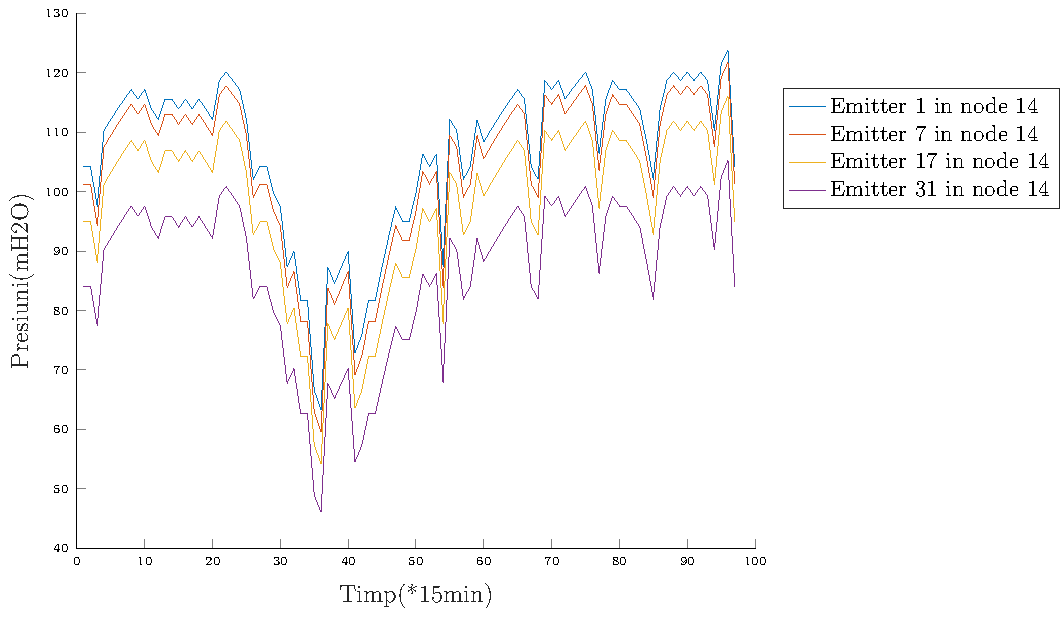
\includegraphics[width=0.5\textwidth]{\pics/c3_pics/emitter_node_same/emitter_node14}%
  \label{fig:emitter_node_same14}%
}\qquad
\subfloat[Profil cu defect în nodul 25]{%
  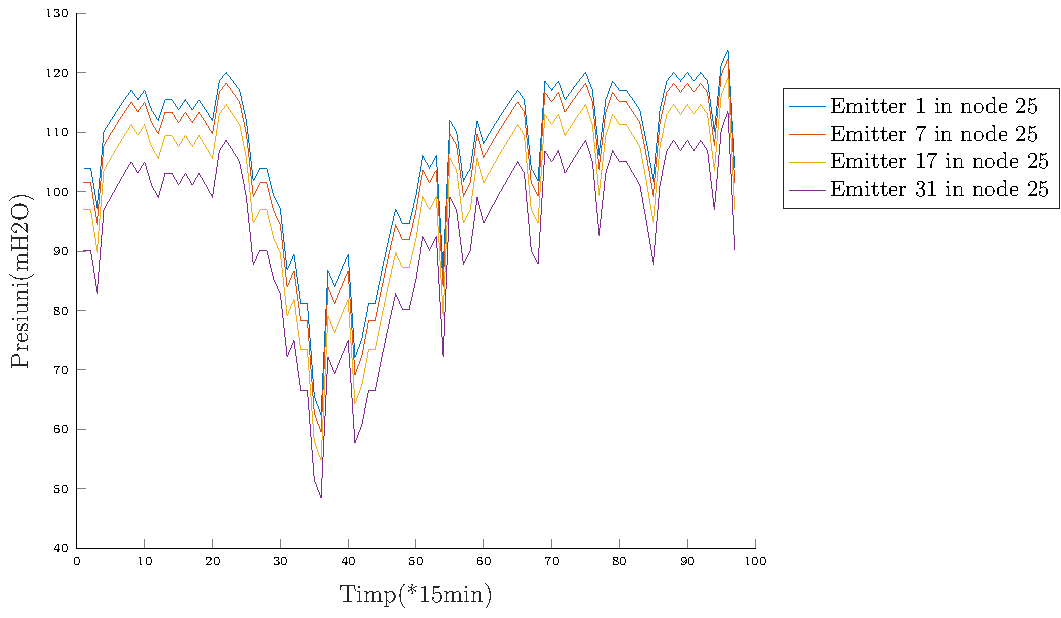
\includegraphics[width=0.5\textwidth]{\pics/c3_pics/emitter_node_same/emitter_node25}%
  \label{fig:emitter_node_same25}\qquad
}

\caption{Rezultate simulări defecte ușoare}
\label{fig:ref_emitter_soft}
\end{figure}

După cum se poate observa în imaginile \ref{fig:ref_emitter_soft} variația emitter-ului într-un nod produce în mod evident o modificarea a modului comun al caracteristicii $timp-presiune$. Din punctul de vedere al magnitudinilor de simulare pentru defecte, am considerat 2 clase de defecte, anume:
\begin{itemize}
\item defecte ușoare (soft faults) - cu valorile coeficientului de emitter mai mici de 35
\item defecte puternice (hard faults) - cu valorile emitter mai mari de 35 
\end{itemize}

Cele din urmă produc și modificări ale caracteristicii dinamice, introducând distorsiuni sau aplatizări ale mărimilor măsurate. Reprezentarea defectelor hard este reprezentată în figurile de mai jos:

\begin{figure}[H]

\subfloat[Profile cu defect puternic în nodul 14]{%
  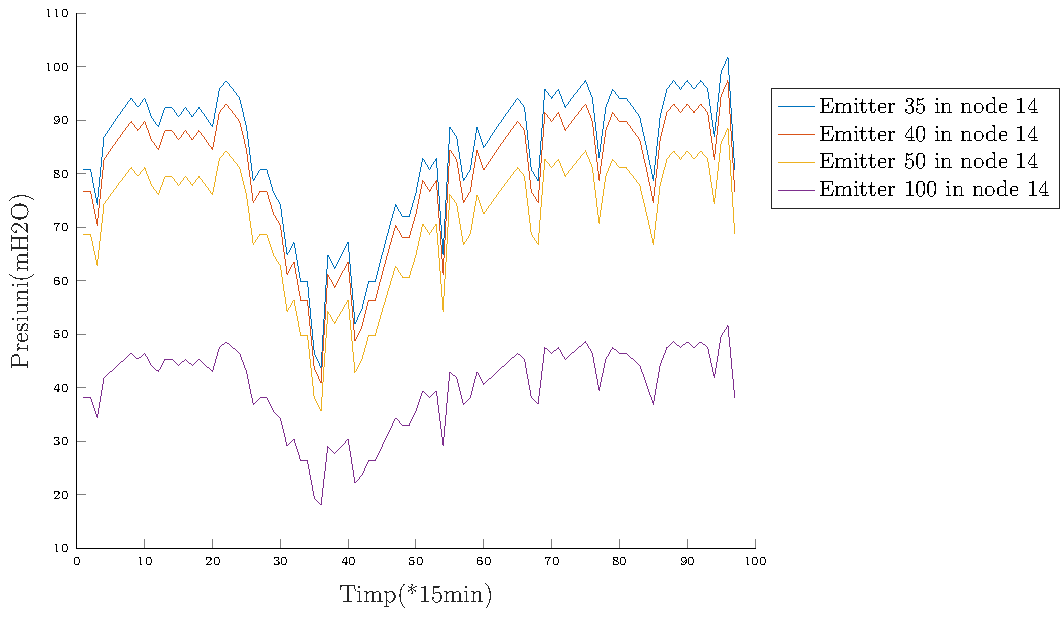
\includegraphics[width=0.5\textwidth]{\pics/c3_pics/emitter_node_same/emitter_hard_node14}%
  \label{fig:emitter_hard_node_same14}%
}\qquad
\subfloat[Profil cu defect puternic în nodul 25]{%
  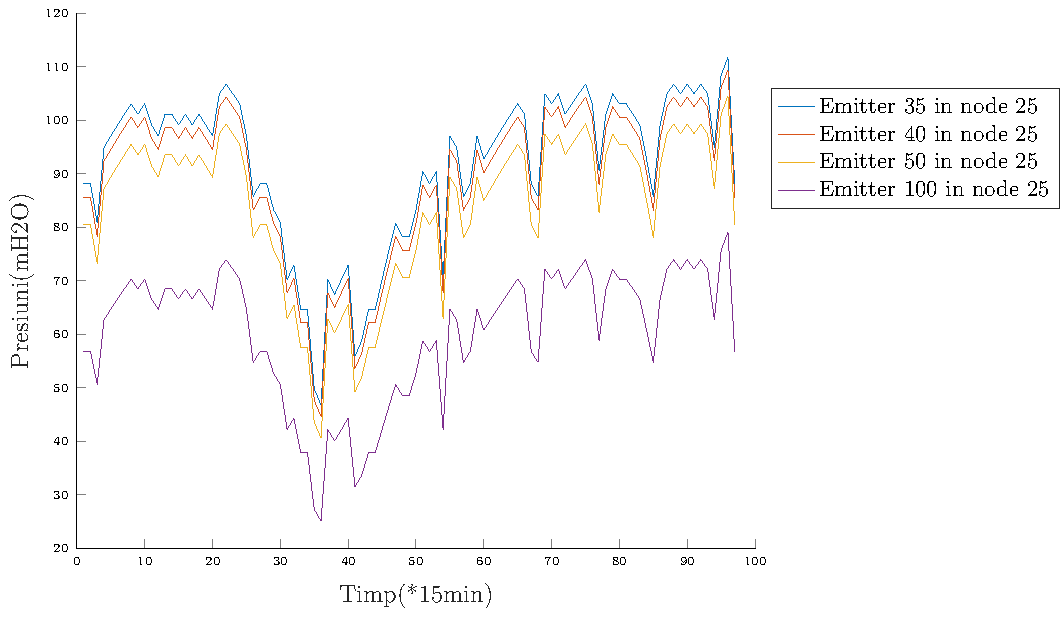
\includegraphics[width=0.5\textwidth]{\pics/c3_pics/emitter_node_same/emitter_hard_node25}%
  \label{fig:emitter_hard_node_same25}\qquad
}
\caption{Rezultate simulări defecte puternice}
\label{fig:ref_emitter_hard}
\end{figure}

Se observă de exemplu că pentru o valoare a emitter-ului de 100 caracteristica dinamică este deja modificată din cauza scurgerilor puternice din nod. 

Este relevantă împărțirea defectelor în mai multe clase de magnitudini pentru a putea valida un model de clasificare. Spre exemplu este normal să se întrebe dacă un model antrenat pe baza unui set date corespunzător unor magnitudini normale $C \in (0, 35)$ poate da rezultate semnificative pentru un set de date cu magnitudini ale emitter-ului puternice $C \geqslant 35$. 

\section{Preprocesarea datelor}
\label{sec:preproc}
În urma extragerii datelor din rețea este extrem de importantă etapa de prelucrare și preprocesare a datelor. Domeniul de preprocesare a datelor este unul extrem de vast și important în domeniul de învățare automată (engl. Machine Learning) și procesare de semnal. Preprocesarea datelor este etapa în care datele de intrare pentru un algoritm sunt aduse la o formă optimă pentru desfășurarea procesului impus, de exemplu în domeniul clasificării este important ca algoritmii să primească date care să fie scalate într-un anumit domeniu, pentru a asigura convergența\cite{dataPreprocessing}, \cite{GIGO}. Alegerea metodei de preprocesare este strâns legată de tipul de date disponibile și de starea acestora. În cazul rețelelor de apă, unde am ales caracteristica presiunii ca mărime de intrare pentru algoritm și ținând cont de răspunsul în timp al rețelei am considerat ca fiind necesare următoarele operații:

\begin{itemize}
\item eliminarea frontului comun și extragerea diferenței dintre semnalul nominal și cel măsurat în rețea
\item filtrarea semnalului obținut anterior
\end{itemize}

\section{Nomenclatura mărimilor alese}
\label{sec:nomenclatura}
Pentru a menține rigurozitatea și eleganța metodelor folosite este nevoie de o definire matematică pentru toate mărimile și metodele de filtrare folosite.

\subsection{Presiunea în regim dinamic}
Reprezintă o funcție de timp:
\begin{equation}
p_i : \mathbb{R} \longrightarrow \mathbb{R}^n, i \in V
\label{eq:press:func}
\end{equation}

unde $n$ reprezintă numărul de noduri al rețelei, iar $i$ reprezintă indexul nodului. 
Deoarece cazurile tratate în această lucrare reprezintă momente discrete de timp este important să definim presiunea măsurată în intervalele discrete în care este simulat procesul:
\begin{equation}
\mathbf{p}_i \in \mathbb{R}^{n \times p_{sim}}
\end{equation}

unde $p_{sim}$ reprezintă numărul de eșantioane pentru fiecare măsurătoare. Mergând mai departe în analiza simulării este de asemenea important să definim mărimea afectată de un defect în nodul $j$, de magnitudine $m$ și măsurată în nodul $i$:
\begin{equation}
\mathbf{p}^{j,m}_i \in \mathbb{R}^{n \times p_{sim}}
\end{equation}

Pentru cazul în care magnitudinea $m$ ia valori nule, atunci vom considera notația mărimii nominale:
\begin{equation}
\mathbf{p}^{j,0}_i = \mathbf{p}^{nom}_i, \forall j \in V
\end{equation}

Pentru valorile presiunii recoltate din rețea în nodul $i$ despre care nu se cunoaște nici o informație, vom considera notația
\begin{equation}
\widehat{\mathbf{p}}_i
\end{equation}

\subsection{Presiunea în regim static}
Considerând o plajă de momente de timp situate între indicii $rs_1 : rs_2$ unde se afla valorile de regim staționar ale procesului, putem defini o medie a regimului static în felul următor:
\begin{equation}
\overline{\mathbf{p}}_i^{j,m} = \frac{1}{rs_1 - rs_2 + 1} \sum_{k=rs_1}^{rs_2} \mathbf{p}_i^{j,m}[k] 
\label{eq:pmean}
\end{equation}

În aceeași manieră definim și media presiunii nominale în regim static:
\begin{equation}
\overline{\mathbf{p}}_i^{j,0} = \overline{\mathbf{p}_i}^{nom}, \forall j \in V
\label{eq:pmean_nom}
\end{equation}

Media presiunii măsurată în nodul $i$ și despre care nu se cunosc informații în legătură cu valoarea și poziția defectului:
\begin{equation}
\overline{\widehat{\mathbf{p}}}_i = \frac{1}{rs_1 - rs_2 + 1} \sum_{k=rs_1}^{rs_2} \widehat{\mathbf{p}}_i^[k] 
\label{eq:pmean_measured}
\end{equation}

\subsection{Reziduuri}
Așa cum a fost discutat în secțiunea \ref{sec:preproc}, preprocesarea datelor are un rol important iar în cazul analizei și clasificării defectelor în rețelele cu apă, este nevoie să definim caracteristica prelucrată care va fi folosită mai apoi în procesul de izolare a defectelor. Reziduul absolut reprezintă diferența dintre valoarea măsurată în rețea și valoarea nominală, aici putem discerne două cazuri:
Reziduu temporal:
\begin{equation}
\mathbf{r}_i^{j,m} = \mathbf{p}_i^{j,m} - \mathbf{p}_i^{nom}
\label{eq:temp_residual}
\end{equation}
Reziduu atemporal, calculat ca diferența dintre cele două valori mediate pe intervalul staționar al caracteristicii:
\begin{equation}
r_i^{j,m} = \overline{\mathbf{p}}_i^{j,m} - \overline{\mathbf{p}}_i^{nom}
\label{eq:absolute_residual}
\end{equation}

iar pentru valorile reziduului despre care nu se cunosc încă lucruri folosim notația din stilul anterior:
\begin{equation}
\widehat{r}_i = \overline{\widehat{\mathbf{p}}}_i - \overline{\mathbf{p}}_i^{nom}
\label{eq:measured_residual}
\end{equation}

Alte tipuri de reziduuri pre-procesate sunt relative:
\begin{equation}
rrelativ_i^{j,m} = \frac{r_i^{j,m}}{\overline{\mathbf{p}}_i^{nom}} 
\label{eq:relative_residual}
\end{equation}

Reziduurile normate:
\begin{equation}
rnorm_{i}^{j,m} =  \frac{r_i^{j,m}}{ \norm{r_{1:n}^{j,m}}} 
\label{eq:norm_residual}
\end{equation}

Reziduurile scalate:
\begin{equation}
rscal_{i}^{j,m} = \frac{r_i^{j,m} - \min r_{1:n}^{j,m}}{ \max r_{1:n}^{j,m} -  \min r_{1:n}^{j,m}}
\label{eq:scaled_residual}
\end{equation}


Ca semnificație notațiile prezentate în \ref{sec:nomenclatura} care conțin simbolul~ $\widehat{}$~ fac referire la datele folosite pentru validarea modelului iar valorile unde se specifică nodul defectului și magnitudinea acestuia sunt considerate ca fiind date de antrenare și testare. Astfel în contextul definirii setului de dat pe care vom aplica algoritmii de clasificare va trebui să definim matricea:
\begin{equation}
\mathbf{R}<tip>^{j, m} \in \mathbb{R}^{n_{d} \times n}
\label{eq:residual_mat}
\end{equation}

Unde croșetele din formulă reprezintă un înlocuitor pentru metoda de reziduu folosită iar $n_{d}$ reprezintă numărul de defecte tratate în setul de date. De asemenea pentru fiecare linie a matricei \eqref{eq:residual_mat} putem defini perechea
\begin{equation}
\left( \mathbf{R}<tip>(d,:), y_{d} \right)
\label{eq:residual_mat_label}
\end{equation} 
Unde $ \mathbf{R}<tip>(d,:)$ reprezintă răspunsul rețelei prin reziduuri la defectul $d$. Iar $y_{d}$ reprezintă eticheta pentru acest set de date, anume, nodul în care a avut loc defectul.

\section{Calcul și prezentare reziduuri}
În continuare vom prezenta grafic reziduurile temporale normalizate care apar în rețea pentru diferite scenarii ale defectelor definite anterior.
Astfel vom considera nodurile de măsurătoare ca o submulțime  a lui $V' \subset V$ și $ V = \{5, 11, 15, 17, 21, 27\}$, nodurile în care s-au simulat defecte sunt $V_{d} = \{11, 17, 27,29\}$.

 
\begin{figure}[H]
\begin{tabular}{cc}
\subfloat[Reziduuri pentru defect în nodul 11, magnitudine 29]{%
  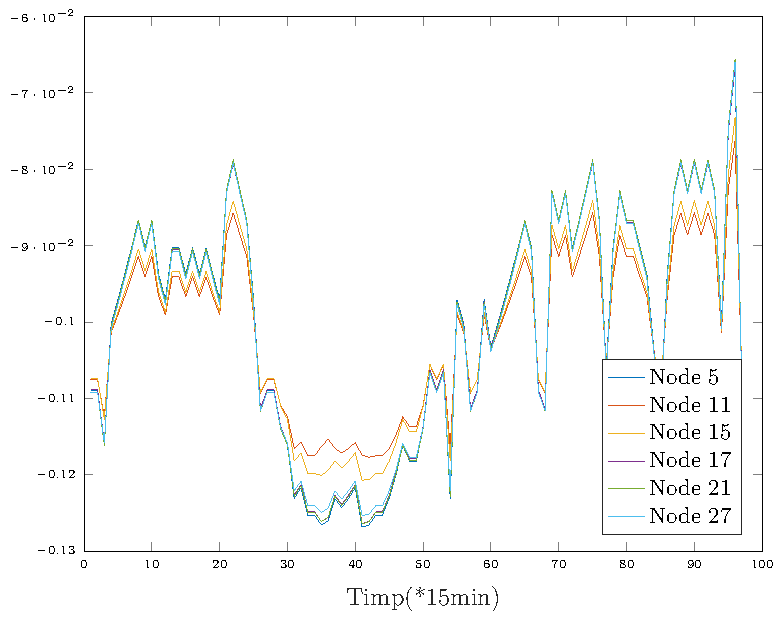
\includegraphics[width=0.5\textwidth]{\pics/c3_pics/residuals/time_res_emitter11_mag29}%
  \label{fig:residual_time_11}%
} &
\subfloat[Reziduuri pentru defect în nodul 17, magnitudine 29]{%
  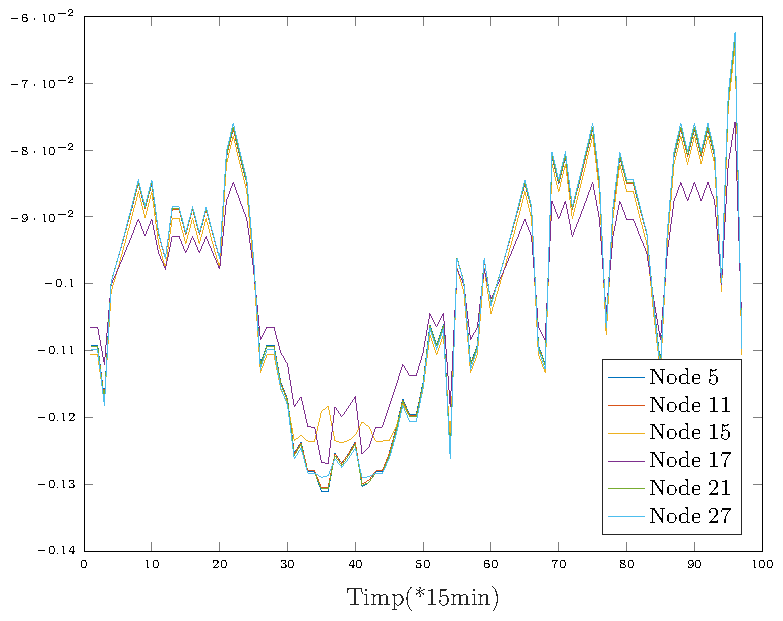
\includegraphics[width=0.5\textwidth]{\pics/c3_pics/residuals/time_res_emitter17_mag29}%
  \label{fig:residual_time_17}%
} \\

\subfloat[Reziduuri pentru defect în nodul 21, magnitudine 29]{%
  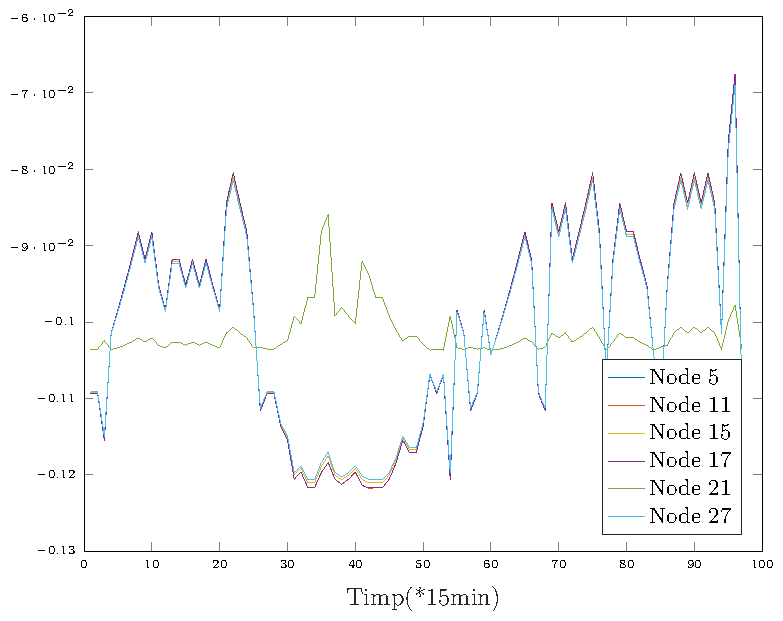
\includegraphics[width=0.5\textwidth]{\pics/c3_pics/residuals/time_res_emitter21_mag29}%
  \label{fig:residual_time_21}%
}&

\subfloat[Reziduuri pentru defect în nodul 27, magnitudine 29]{%
  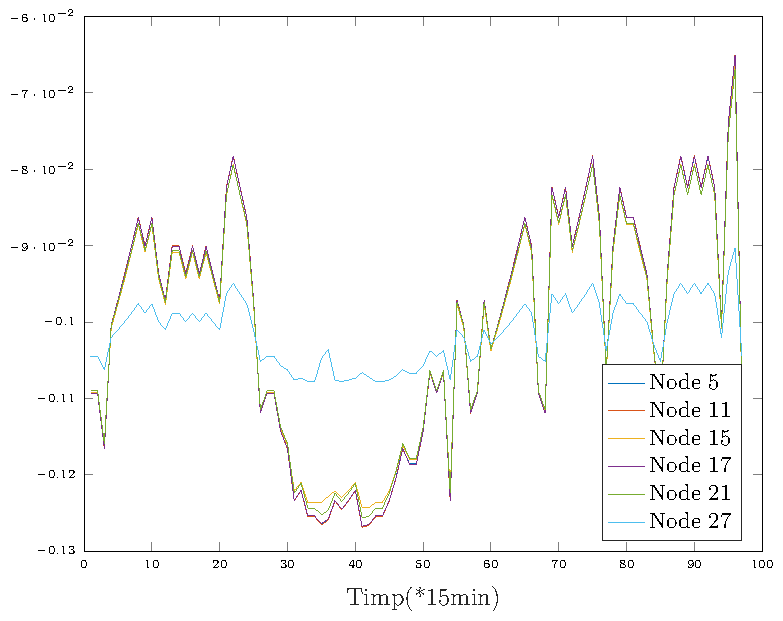
\includegraphics[width=0.5\textwidth]{\pics/c3_pics/residuals/time_res_emitter27_mag29}%
  \label{fig:residual_time_27}%
} 
\end{tabular}
\caption{Reziduuri rețea}
\label{fig:rez_time}
\end{figure}


Se poate observa că în figurile \ref{fig:rez_time} reziduul cel mai pronunțat ca funcție de timp se găsește în nodul în care se simulează și defectul - lucru natural și de așteptat. O caracteristică importantă a acestei rețele de apă este faptul că există o dependență între diferitele răspunsuri în timp ale caracteristicii de presiune, fapt care ne permite să exploatăm redundanțele din rețea și să prezicem cu o acuratețe relativ ridicată defectele.

Este necesar acum să prezentăm profilurile reziduurilor atemporale, care în final vor reprezenta caracteristicile de intrare pentru algoritmul de clasificare și selecție de senzori.

\begin{figure}[H]
\begin{tabular}{cc}
\subfloat[Reziduuri pentru defect în nodul 11, magnitudine 25]{%
  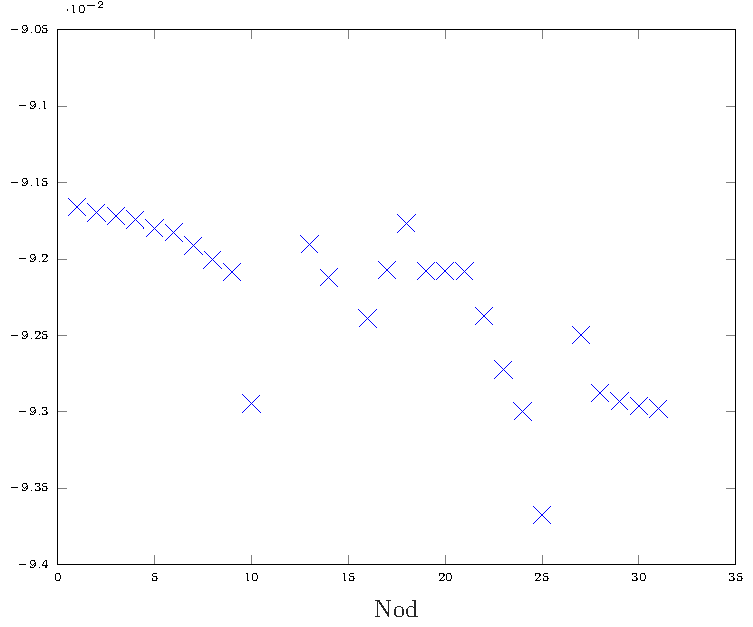
\includegraphics[width=0.5\textwidth]{\pics/c3_pics/residuals/atem_res_emitter11_mag25}%
  \label{fig:residual_atemp_11}%
} &
\subfloat[Reziduuri pentru defect în nodul 17, magnitudine 25]{%
  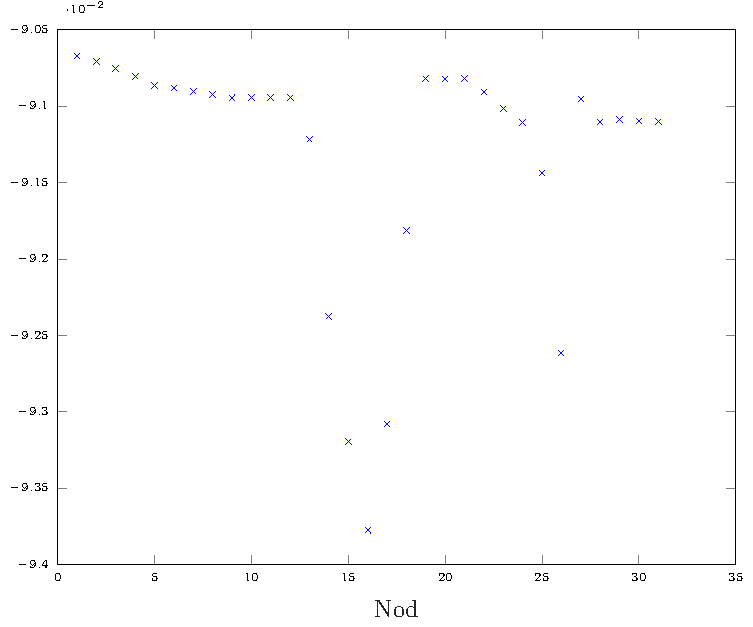
\includegraphics[width=0.5\textwidth]{\pics/c3_pics/residuals/atem_res_emitter17_mag25}%
  \label{fig:residual_atemp_17}%
} \\

\subfloat[Reziduuri pentru defect în nodul 21, magnitudine 25]{%
  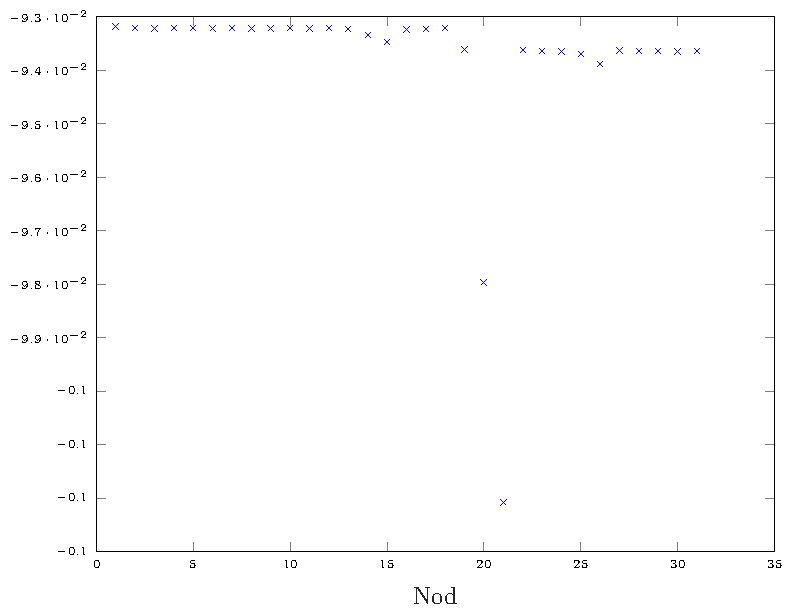
\includegraphics[width=0.5\textwidth]{\pics/c3_pics/residuals/atem_res_emitter21_mag25}%
  \label{fig:residual_atemp_21}%
}&

\subfloat[Reziduuri pentru defect în nodul 27, magnitudine 25]{%
  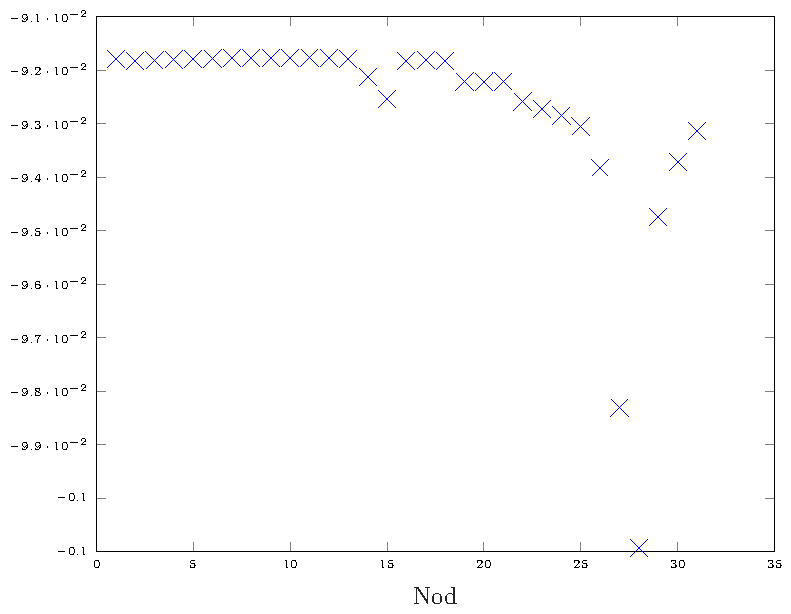
\includegraphics[width=0.5\textwidth]{\pics/c3_pics/residuals/atem_res_emitter27_mag25}%
  \label{fig:residual_atemp_27}%
} 
\end{tabular}
\caption{Reziduuri atemporale rețea}
\label{fig:rez_atemp}
\end{figure}

Asemenea reziduurilor de la \ref{fig:rez_time} se poate observa că simularea unui emitter într-un nod va determina un răspuns puternic în nodul respectiv și în vecinătatea nodului afectat

\section{Metodă preliminară de selecție a senzorilor}
O metodă prin care se poate decide și evalua importanța senzorilor într-o rețea este prin construirea matricei de reziduuri \eqref{eq:residual_mat}, asupra căreia aplicăm o operație de scalare pe coloane, pentru a aduce valorile acesteia în intervalul $[0,1]$. Pentru experimentul în care simulăm în fiecare nod un emitter de 25 obținem grafic o matrice $\mathbf{R}scaled \in \mathbb{R}^{31 \times 31}$:

\begin{figure}[H]
\centering

\includegraphics[width=0.85\textwidth]{\pics/c3_pics/residuals/residual_scaled_matrix}
\caption{Matricea de reziduuri scalate}
\label{fig:rez_scaled_matrix_img}
\end{figure} 

După cum se observă în \ref{fig:rez_scaled_matrix_img} fiecare coloană a matricei $\mathbf{R}scaled$ reprezintă răspunsul prelucrat - scalat în intervalul $[0,1]$ - al unui defect, valorile care tind spre o culoare mai închisă de negru sunt răspunsuri mai pronunțate iar valorile care se apropie de alb reprezintă valori mai puțin evidențiate ale reziduului în nod. Analizând matricea se poate observa care noduri răspund mai bine la anumite răspunsuri, o caracteristică importantă a acestei matrice este că, o alură diagonală - semnificația elementelor diagonale fiind răspunsul nodurilor afectate de defecte aplicate în ele însuși. Dacă matricea de reziduuri ar fi avut o caracteristică diagonală perfectă - elementele nenule s-ar fi regăsit doar pe aceasta - problema de clasificare ar fi fost una simplă și ar fi implicat amplasarea unui senzor în fiecare nod. Cazul real impune dependențe între presiunile, debitele din fiecare nod, dar și vitezele din fiecare conductă, astfel, fiecare defect separat va avea o "amprentă" unică - prin care se diferențiază de celelalte și una comună. Scopul este găsirea unui subset al mulțimii de noduri care să poată identifica defectele cu pierderi minime de performanțe.


\subsection{Binarizarea matricei de reziduuri}

Pentru a putea reține un răspuns binar în cadrul matricei este important să considerăm o limită $l$ peste care răspunsul senzorului este luat în considerare sau nu. Astfel definim matricea binară $\mathbf{M}$ de aceeași dimensiune ca și $\mathbf{R}scaled$ dar peste care aplicăm o operație de binarizare:

\begin{equation}
    \mathbf{M}_{i,j} = \begin{cases}
            1 &\quad \text{ dacă } \mathbf{R}scaled_{i,j} \geq l \\
            0 &\quad \text{ dacă } \mathbf{R}scaled_{i,j}  < l
    \end{cases}
\end{equation}
În continuare vom defini notațiile matematice pentru mulțimile defectelor și a nodurilor.
Este important să considerăm astfel mulțimea răspunsurilor la defecte $F = \{\mathbf{f}_i | i \in V \}$ iar fiecare element $\mathbf{f}_i$ al mulțimii este definit ca un vector format din valori binare cu însemnătatea:

\begin{equation}
\mathbf{f}_i[k] = \begin{cases}
       1 &\quad\text{dacă nodul k răspunde la defectul i}\\
       0 &\quad\text{dacă nodul k nu răspunde la defectul i}
     \end{cases}
\label{eq:fault_signature}
\end{equation}

Echivalent putem defini mulțimea răspunsurilor nodurilor $N =\{\mathbf{n}_i| i \in V\}$, pentru fiecare element $\mathbf{n}_i$ avem:

\begin{equation}
\mathbf{n}_i[k] = \begin{cases}
       1 &\quad\text{dacă defectul k este detectat de nodul k}\\
       0 &\quad\text{dacă defectul k nu este detectat de nodul k}
     \end{cases}
\label{eq:fault_signature}
\end{equation}

todo adauga grafic cu matricea binara M


\subsection{Selecția senzorilor}

Având definite elementele pentru interpretarea decizională a datelor preluate de la senzori, putem formula o metodă prin care să selectăm acei senzori care oferă informațiile cele mai importante. După cum se observă și în matricea reziduurilor \ref{fig:rez_scaled_matrix_img} există foarte multă redundanță în sistemul complex al rețelei de apă care întâmpină perturbații precum scurgeri. Ținând cont că de faptul că fiecare defect are un răspuns diferit, putem să decidem care este subsetul de senzori care reușește să ofere informații îndeajuns de relevante în legătură cu evenimentele din rețea, ca exemplu trivial putem afirma că un nod care răspunde la toate defectele oferă informații relevante pentru detecția de defecte dar nu și pentru izolarea defectelor.

Pentru problema selecției de senzori dorim să obținem o submulțime de noduri $V_s \subset V^j$ cu proprietatea că aceasta va avea un cardinal cât mai mic și defectele detectate de senzorii selectați sunt cât mai multe. Problema aceasta reprezintă de fapt o abordare a unei probleme NP-complete anume Minimum Set Cover - problema acoperirii minime a mulțimilor \cite{perelman2016sensor}.

\paragraph{Problema MSC} \mbox{} \\
Fiind dată o mulțime univers $U$ cu $|U| = n$ și o mulțime cu cardinal $m$ $S = \{S_i | S_i \subset U\}$ având proprietatea că  $\bigcup\limits_{i=1}^{m} S_{i} = U$ se dorește găsirea celei mai mici partiții a mulțimii $S$ a cărei reuniuni va fi egală cu $U$ \cite{CLRS}. 

În cazul rețelelor de apă mulțimea $U$ reprezintă de fapt mulțimea defectelor pentru care se dorește găsirea partiției cu cardinal minim a mulțimii de noduri care să fie sensibilă la toate defectele \cite{perelman2016sensor}.

Această problemă poate fi pusă sub forma unei probleme de optimizare matematică, având la dispoziție matricea binară $\mathbf{M}$ și un vector de selecție a senzorilor $\alpha$:
% \begin{equation*}
% \begin{align}
%     &\min_{\alpha \in \mathbb{R}^n} \sum_{j} \alpha_{j} \\
%     & s.l.: \sum_{j} M_{i,j}\alpha_{j} \geq 1,  i = \overline{1,n_{faults}}
% \end{align}
% \end{equation*}

\begin{subequations}
\begin{alignat}{2}
&\!\min_{\alpha \in \mathbb{R}^n}        &\qquad& \sum_{j} \alpha_{j} \label{eq:optProb}\\
&\text{s.l.:} &      & \sum_{j} M_{i,j}\alpha_{j} \geq 1 \label{eq:constr}
\end{alignat}
\end{subequations}

 Minimizarea sumei vectorului $\alpha$ din \ref{eq:optProb} se referă la selectarea unui număr cât mai mic de senzori pentru a fi plasați în rețea. Constrângerea atașată acestei probleme de programare liniară \eqref{eq:constr} are rolul de a impune ca pentru fiecare defect să existe cel puțin un senzor care să îl detecteze.
 
 todo adaug codul de matlab pentru sensor detection si sa prezint nodurile alese, imaginea retelei cu nodurile selectate încercuite cu portocaliu
 
 ploturi cu reziduurile in nodurile alese de problema de optimizare 
 
 todo adaug plots cu senzorii selectati idk
\chapter{Clasificarea defectelor folosind tehnici de învățare automată}
\label{chap:ml_classification}


\section{Problematica domeniului de învățare automată}
Învățarea automată reprezintă un subdomeniu al inteligenței artificiale, știința care se ocupă cu dezvoltarea de algoritmi care să transpună în domeniul mașinilor acele sarcini care sunt ușor de făcut pentru om, spre exemplu: interpretarea limbajului natural și a imaginilor, recunoașterea obiectelor, menținerea echilibrului sau luarea de decizii. Deși aceste acțiuni par destul banale pentru un om, pentru un computer problema este foarte greu de definit pentru a putea da rezultate relevante.

\section{Mașini cu vectori suport}

\section{Rezultate preliminare folosind toți senzorii}

\section{Selecția de senzori folosind Eliminarea recursivă de caracteristici}

\section{Rezultate folosind senzorii selectați}
\chapter{Clasificarea defectelor folosind metoda învățării de dicționare rare}
\label{chap:dictionary_learning}
\section{Aspecte teoretice}
Problema învățării dicționarelor se clasează în domeniul problemelor de învățare nesupervizată - setul de date nu trebuie să fie structurat pe clase - dar există și variațiuni ale acesteia prin care modifică problema de optimizare astfel încât să se poată învăța dicționare specializate pentru clasificare.

Având ca date de intrare un set de date $\mathbf{Y} \in \mathbb{R}^{n \times n_s}$, unde $n$ reprezintă dimensiunea semnalelor și $n_s$ reprezintă numărul de semnale folosite la antrenare, dorim să găsim acele matrice $\mathbf{D} \in \mathbb{R}^{n \times m}$ și $\mathbf{X} \in \mathbb{R}^{m \times n_s}$ astfel încât să rezolvăm problema de optimizare\cite[Capitol 2]{DL_book}:

\begin{subequations}
\begin{alignat}{2}
&\!\min_{\mathbf{D}, \mathbf{R}}        &\qquad& ||\mathbf{Y} - \mathbf{D} \mathbf{X} ||^{2}_{F} \label{eq:dl_opt}\\
&\text{s.l.:} &      & ||x_l||_0  \leq s, l = 1:N \label{eq:dl_sparsity}\\
& & & ||d_j|| = 1, j = 1:n \label{eq:dl_norm}
\end{alignat}
\label{eq:dl_opt_problem}
\end{subequations}
Unde:
\begin{itemize}
    \item $\mathbf{D}$ reprezintă matricea dicționarului pe baza căruia se va calcula reprezentarea, coloanele acesteia se numesc atomi
    \item $\mathbf{X}$ este reprezentarea rară a setului de date $\mathbf{Y}$
\end{itemize}

Constrângerea \eqref{eq:dl_sparsity} se referă la raritatea vectorului de reprezentare iar \eqref{eq:dl_norm} la normalizarea atomilor pentru dicționar.

Problema de găsire a dicționarului și a reprezentării semnalelor de antrenare $\mathbf{Y}$ conține neliniarități puternice din cauza condiției de sparsitate impuse. Cazul interesant și cel mai abordat în literatură îl reprezintă acela în care dicționarul este supracomplet \cite[Capitolul 1]{DL_book}, această proprietate poate aduce numeroase beneficii diferitelor procese de clasificare, anume:
\begin{itemize}
    \item stocarea matricelor sparse se face mult mai eficient decât cele pline
    \item din punct de vedere computațional există foarte multe multiplicări care nu se vor mai efectua
\end{itemize}

Modul în care am descris problema duce cu gândul la o metodă sofisticată de extragere a caracteristicilor din setul de date. Astfel dacă extragem o reprezentare sparsă $X = \{x_i\}$, putem să folosim vectorul rar $x_i$ ca exemplu de antrenare pentru alți algoritmi de antrenare sau clasificare.


\subsection{Găsirea reprezentării sparse}
Reprezentarea sparsă se ocupă de reconstruirea unui semnal $y \in \mathbf{R}^n$ având la dispoziție un dicționar $\mb{D} \in \mathbb{R}^{n\times m}, \mb{D} = [d_1, d_2, ..., d_m]$ cu $m > n$, adică, găsirea unui vector $\mb{x} \in \mathbb{R}^m$ astfel încât $y \approx \mb{D} \mb{x}$. 
Reziduul aproximării sparse este definit ca:

\begin{equation}
    e = y - \mb{D} \mb{x}
\end{equation}

Un algoritm greedy care rezolvă această problemă este OMP \textit{Orthogonal Mathching Pursuit}. Având la un moment dat mulțimea $\mathcal{S}$ a atomilor din dicționar selectați, algoritmul dorește să atingă un anumit nivel de sparsitate $s = |\mathcal{S}|$ și îndeplinirea unui criteriu de eroare $||y - \mb{D_{\mathcal{S}}} \mb{x}|| < tol$ \cite[Capitolul 1]{DL_book}. Algoritmul va completa mulțimea $\mathcal{S}$  cu acel atom $d_k$ care nu se află în ea și care va fi cel mai bine corelat cu reziduul actual, deci $k = arg \max_{j \not \in \mathcal{S}} |e^T x_j|$. 

Pentru a putea obține reprezentarea semnalului $y$ folosind mulțimea de atomi $\mathcal{S}$ este nevoie să rezolvăm sistemul de ecuații supradeterminat:

\begin{equation}
    \mb{D} \mb{x} = \mb{y}
\end{equation}

Prin folosirea soluției ecuațiilor normale:

\begin{equation}
    \mb{x} = (\mb{D} \mb{D}^T)^{-1} \mb{D} \mb{y}
\end{equation}


\section{Adaptarea la problema rețelelor de apă}

Pentru a putea clasifica nodurile unde s-au produs defecte trebuie extinsă problema de optimizare \eqref{eq:dl_opt_problem} astfel încât să se ia în calcul o structură eficientă a dicționarului pentru reprezentarea sparsă a reziduurilor, dar și apariția unei noi matrici $\mathbf{W}$ numită clasificator \cite{DL_book}:
\begin{equation}
    \min_{\mathbf{W}} || \mathbf{H} - \mathbf{W}\mathbf{X}||_F^{2} + \gamma ||\mathbf{W}||^2_F
    \label{eq:dl_nmf}
\end{equation}

matricea $\mathbf{H}$ reprezintă colecția de etichete pentru fiecare dintre reziduurile din $\mathbf{Y}$
forma lui fiind:

\begin{equation}
    \mathbf{H}_i = e_k, \text{dacă pentru exemplul i s-a produs un defect în nodul k}
    \label{eq:struct_H}
\end{equation}

parametrul $\gamma$ are rolul de a condiționa mai bine matricea și a evita fenomenul de \textit{overfitting}.
Matricea $\mathbf{W}$ reprezintă o matrice de transformare care în mod ideal încearcă să transforme spațiul rar $\mathbf{X}$ într-un spațiu categoric de tipul versorilor $e_k \in \mathbb{R}^{n_{clase}}$. Real vorbind, ceea ce se întâmplă este că rezultatul înmulțirii $\mathbf{W}\mathbf{X}$ este un vector dens, unde indexul celui mai mare element denotă de fapt clasa din care face parte reziduul transformat $p_{dl} = argmax(\mathbf{W}\mathbf{x})$ \cite[Capitolul 8]{DL_book}. 
Agregând cele două probleme de optimizare obținem învățarea de dicționare discriminative:

\begin{equation}
    \min_{\mathbf{D}, \mathbf{X}, \mathbf{W}} || \mathbf{Y} - \mathbf{D} \mathbf{X} ||^2_F + \alpha || \mathbf{H} - \mathbf{W} \mathbf{X} ||^2_F
    \label{eq:disc_DL}
\end{equation}


O altă modalitate e a spori performanțele de clasificare este prin obligarea problemei de optimizare să aloce anumiți atomi ai dicționarului $\mathbf{D}$ unor anumite clase de defecte - învățarea de dicționare cu consistență de clasă \textit{label consistent dictionary learning} \cite{DL_book}. Problema de optimizare la care se reduce este:

\begin{equation}
    \min_{\mb{D}, \mb{W}, \mb{A}, \mb{X}} || \mb{Y} - \mb{D}\mb{X}||^2_F + \alpha ||\mb{H} - \mb{W} \mb{X} ||^2_F + \beta ||\mb{Q} - \mb{A}\mb{X} ||^2_F
    \label{eq:lc_dl}
\end{equation}

matricea $\mb{Q}$ fiind de fapt parametrul care alocă fiecare atom unui anumit defect și contribuie la sporirea calității clasificării. Liniile matricei $\mb{Q}$ sunt asociate fiecărui atom cu proprietatea

\begin{equation}
    q_{ij} = \begin{cases}
    1,\quad \text{atomul i este asociat clasei j} \\
    0,\quad  \text{în rest}
    \end{cases}
\end{equation}

Problema \eqref{eq:lc_dl} poate fi redusă la problema de optimizare \cite{DL_book}:

\begin{equation}
    \min_{\mb{D}, \mb{W}, \mb{A}, \mb{X}} 
    \norm{
    \begin{bmatrix}
    \mb{Y} \\
    \sqrt{\alpha} \mb{H} \\
    \sqrt{\beta} \mb{Q}
    \end{bmatrix}
    -
     \begin{bmatrix}
    \mb{D} \\
    \sqrt{\alpha} \mb{W}\\
    \sqrt{\beta} \mb{A}
    \end{bmatrix} 
    \mb{X}
    }^2_F
    \label{eq:lc_dl}
\end{equation}

și poate fi rezolvată cu ajutorul algoritmului K-DVS care funcționează prin alternarea fixării matricelor $\mb{D}$ și $\mb{X}$, prima dată dicționarul este fixat și se găsește cea mai bună reprezentare $\mb{X}$, apoi se recalculează dicționarul $\mb{D}$. Metoda se bazează pe aproximarea unei matrice de rang n printr-o sumă de matrice de rang 1.





\section{Rezultate și metrici de clasificare}

Pentru testarea metodelor de DL am folosit setul de date de la capitolul \ref{chap:ml_classification}, iar metodele care calculează dicționarele și reprezentările sparse sunt cele de la \cite{dl-code}. Asemănător capitolului de clasificare cu SVM voi considera nodurile alese prin metoda MSC și prin metoda RFE, și voi arăta pentru fiecare dintre acestea acuratețea obținută cu ajutorul metodelor de DL cu consistență de clasă și DL discriminativ.
Astfel avem pentru senzorii selectați de algoritmul RFE:
\begin{table}
    \centering
    \begin{tabular}{|c|c|c|c|}
    \hline
         Nr senzori & Senzori selectați & Acuratețe DL discriminativ & Acuratețe LC-DL \\
        \hline

        4 & $10, 11, 25, 27$ & $46.5\%$ & $82.4\%$\\
        \hline
        6 & $10, 11, 16, 25, 27, 28$ & $53.1\%$ & $86.2\%$ \\
        \hline
        10 & $ 9, 10, 11, 12, 16, 20, 25, 27, 28, 29 $ & $57.2\%$ & $93.3\%$  \\
        \hline
    \end{tabular}
    \caption{Performanțele clasificării DL cu senzorii selectați de RFE}
    \label{tab:dl_rfe_performance}
\end{table}
Iar pentru metoda de plasare a senzorilor cu problema MSC am obținut rezultatele:

\begin{table}[H]
    \centering
    \begin{tabular}{|c|c|c|c|}
    \hline
        Nr senzori & Senzori selectați & Acuratețe DL discriminativ & Acuratețe LC-DL \\
        \hline
        4 & $11, 15, 21, 28$ & $58.7\%$ & $89.7\%$ \\
        \hline
        6 & $12, 13, 16, 21, 25 , 26 $ & $51.4\%$ & $86.9\%$\\
        \hline
        10 & $6,12,13,14,15,16,21,26,27, 28$ & $65.59\%$ & $96.7\%$\\
        \hline
    \end{tabular}
    \caption{Performanțele clasificării DL cu senzorii selectați de MSC}
    \label{tab:dl_msc_performance}
\end{table}


Luând în calcul cei 10 senzori selectați de metoda MSC clasificatorul obținut de metoda învățarii de dicționare cu consistență de clase dă un rezultat al acurateții de 96.7\%, cu 2.3 \% mai performant decât abordarea cu SVM. Astfel putem afirma că învățare dicționarelor rare poate fi aplicată cu succes în problema clasificării defectelor într-o rețea cu apă și în principiu oferă o așa zisă robustețe, deoarece atomii asignați unei anumite clase vor reprezenta într-un mod prost profilurile defectelor din altă clasă.




\chapter{Concluzii și direcții viitoare}
\label{chap:conclusions}

În această lucrare am prezentat problematica identificării defectelor într-o rețea de apă, prin analiza profilurilor reziduurilor într-o perioadă de timp corespunzătoare regimului staționar. Abordarea s-a axat pe alegerea unei metode empirice și statistice în detrimentul unei metode analitice, așa cum a fost prezentat și în capitolul \ref{chap:simulari}, o interpretare exactă a rețelelor de apă este zadarnică, procesul care stă în spatele dependenței presiune - debit - viteză în conducte fiind unul puternic neliniar și influențat de mulți factori exogeni. 

Abordarea propusă în această lucrare este una bine documentată \cite{irofti2017dictionary}, \cite{perelman2016sensor}, \cite{rossman2000epanet} asupra căreia am aplicat două metode de învățare automată supervizată - mașini cu vectori suport și învățarea de dicționare rare. De asemenea o preocupare a acestei lucrări a fost centrată asupra optimizării procesului de clasificare, anume reducerea numărului de senzori prezenți la clasificare. Motivația reducerii numărului de senzori este ajungerea la un compromis ingineresc între investiția în senzorii plasați în nodurile rețelei de apă și cheltuielile pentru combaterea defectelor. Rezultatul reducerii numărului de senzori prin metoda \ref{alg:rfe} și prin rezolvarea problemei NP-Complete \ref{eq:opt_problem}, a arătat prezența redundanței puternice între informațiile provenite de la senzori, în mod natural, deoarece nodurile vecine într-un graf sunt supuse unor solicitări foarte apropiate.

Rezultatele clasificării folosind metodele LC-DL și SVM au dat rezultate apreciabile și relevante din punct de vedere statistic, antrenarea și testarea fiind făcută pe două seturi de date echilibrate (i.e. același număr de obiecte pentru fiecare clasă) și variate - fiecare defect pentru care se încerca clasificarea avea ca exemple de clasă profiluri cu mai multe magnitudini - metricile de acuratețe atingând un procent foarte ridicat - 96.7\% pentru LC-DL folosind 10 senzori aleși cu MSC și 94.1\% pentru SVM folosind 10 senzori aleși cu RFE. De asemenea algoritmul SVM poate fi folosit într-un alt algoritm \ref{alg:rfe} pentru a putea alege nodurile din rețea cu cea mai importantă contribuție.

\begin{figure}[H]
\centering
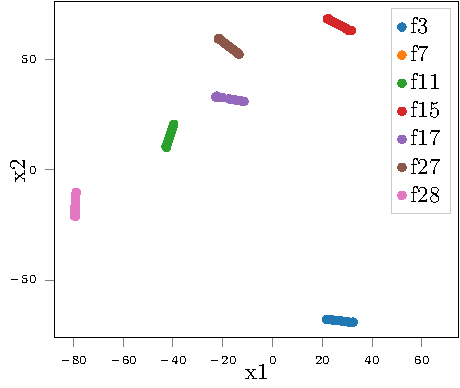
\includegraphics[width=0.45\textwidth]{\pics/c6_pics/2dfaults}
\caption{Proiecția în 2D a profilurilor defectelor}
\label{fig:tsne_faults}
\end{figure}

Ca ilustrație grafică bidimensională asupra profilurilor defectelor am realizat în figura \ref{fig:tsne_faults} proiecția pe 2 axe a vectorului de caracteristici al unui defect format din 31 de caracteristici, folosind algoritmul TSNE. După cum se poate observa aceste defecte nu numai ca sunt liniar separabile, dar în funcție de magnitudinea emițătorului în nodul respectiv proiecțiile $(x1, x2)$ se vor situa pe o dreaptă. Deși folosirea unei metode de clasificarea bazate pe extragerea proiecțiilor în 2D sau 3D prin algoritmul TSNE poate părea o idee atractivă, problema apare în momentul în care se dorește transformarea unui set de date nou - fiind un algoritm stocastic TSNE va da rezultate diferite la fiecare rulare și există riscul ca aceleași defecte să fie coagulate în alte zone ale planului bidimensional, compromițând astfel procesul de clasificare.




%%%%%%%%%%%%%%%%%%%%%% back matter %%%%%%%%%%%%%%%%%%%%%%%%%%%%%%%%%%%%%%
\appendix
\appendixpage
%\addappheadtotoc
\begin{appendices}																				  % from here onwards are the appendices
%\chapter{Notaţii matematice consacrate}
\label{chap:not}

\begin{description}[style=nextline]
\item[Constante scalare] $\mathrm{a}$, $\mathrm{A}$, $\mathrm{b}$, $\mathrm{B}$, $\mathrm{c}$, $\mathrm{C}$ etc. (litere normale, cu precădere din prima parte a alfabetului);
\item[Constante vectoriale] $\mathbf{a}$, $\mathbf{b}$, $\mathbf{c}$ etc. (litere minuscule, aldine (\textbf{bold}), cu precădere din prima parte a alfabetului);
\item[Constante matriciale] $\mathbf{A}$, $\mathbf{B}$, $\mathbf{C}$, $\mathbf{P}$, $\mathbf{Q}$, $\mathbf{R}$ etc. (litere majuscule, aldine (\textbf{bold}), cu precădere din zona alfabetului unde nu se afl\u a litere alocate în mod tradi\c tional indicilor);
\item[Variabile scalare] $x$, $y$, $z$  etc. (aplecate (\emph{italic}), ne-aldine, cu prec\u adere din ultima parte a alfabetului);
\item[Variabile vectoriale] $\mathbf{x}$, $\mathbf{y}$, $\mathbf{z}$ etc (litere minuscule, aldine (\textbf{bold}), cu precădere din ultima parte a alfabetului);
\item[Variabile  matriciale]  $\mathbf H(q^{-1})$, $\mathbf H(s)$, $\mathbf H(z)$, $\mathbf H(t)$, $\mathbf H[k]$ etc. (litere  majuscule,  aldine (\textbf{bold}), cu unul sau mai multe argumente scalare sau vectoriale);
\item[Operatori]  $\min$ (minim), $\max$ (maxim), opt (optim), $\arg$ opt (argument de optimizare sau punct de optimizare), $q^{-1}$  (întârziere), $Tr$ (urmă (\emph{trace})), $Tz$ (Toeplitz), $Pr$ (proiec\c tie) etc, (litere normale, urmate obligatoriu de explica\c tia privind nota\c tia, la prima utilizare);
\item[Timp continuu] $t\in \mathbb R$;
\item[Timp discret] $n\in \mathbb Z$ sau $k\in \mathbb Z$;
\item[Argument de timp continuu] $(t)$ (între parenteze rotunde);
\item[Argument de timp discret] $[n]$ (între paranteze drepte);
\item[Număr de itera\c tie sau indici] $i$, $j$, $k$, $l$, $m$, $n$  etc. (aplecate, cu precădere din partea de mijloc a alfabetului); exemplu de nota\c tie complex\u a": $x_i^k[n]$ -- componenta $i$ a vectorului $\mathbf x$, la momentul discret $n$, pentru iteratia $k$;
\item[Caractere greceşti frecvent utilizate (în ordinea firească a alfabetului grecesc)]~
\begin{itemize}
\item $\alpha$ (/alfa/, \verb+\alpha+)
\item $\beta$ (/beta/, \verb+\beta+)
\item $\gamma$, $\Gamma$ (/gama/, \verb+\gamma, \Gamma+)
\item $\delta$, $\Delta$ (/delta/, \verb+\delta, \Delta+)
\item $\epsilon$ (/epsilon/, \verb+\epsilon+)
\item $\zeta$ (/\c teta/, \verb+\zeta+)
\item $\eta$ (/ita/, \verb+\eta+)
\item $\theta$, $\Theta$ (/teta/, \verb+\theta, \Theta+)
\item $\kappa$ (/kapa/, \verb+\kappa+)
\item $\lambda$, $\Lambda$ (/lambda/, \verb+\lambda, \Lambda+) a nu se pronun\c ta /lamda/
\item $\mu$ (/miu/, \verb+\mu+)
\item $\nu$ (/niu/, \verb+\nu+)
\item $\xi$ (/xi/, \verb+\xi+)
\item $\pi$, $\Pi$ (/pi/, \verb+\pi, \Pi+)
\item $\rho$ (/ro/, \verb+\rho+)
\item $\sigma$, $\Sigma$ (/sigma/, \verb+\sigma, \Sigma+)
\item $\tau$ (/tau/, \verb+\tau+)
\item $\phi$, $\varphi$, $\Phi$ (/fi/, \verb+\phi, \varphi, \Phi+)
\item $\chi$ (/hi/, \verb+\chi+)
\item $\psi$, $\Psi$ (/psi/, \verb+\psi, \Psi+)
\item $\omega$, $\Omega$ (/omega/, \verb+\omega, \Omega+)
\end{itemize}
Şi  în  cazul  lor,  se  vor  respecta  regulile  de  nota\c tie  pentru  scalari/vectori. % Totuşi,  în  cazul scalarilor, se recomandă ca literele să nu fie scrise aplecat. De exemplu, se va prefera  $\mathrm \alpha$ şi nu $\alpha$.
\item[Alte nota\c tii unificate în Automatică]~
\begin{description}[before={\renewcommand\makelabel[1]{##1 =}},leftmargin=!,labelwidth=\widthof{\bfseries blaaaaaaaa}]
\item[$J$, $\mathbf J$] criteriu (de optimizare), func\c tie-criteriu, (func\c tie) cost, func\c tie economică, func\c tie obiectiv
\item[$u$, $\mathbf u$] intrarea/comanda (scalară sau vectorială a) unui sistem dinamic
\item[$x$, $\mathbf x$] starea (scalară sau vectorială a) unui sistem dinamic
\item[$y$, $\mathbf y$] ieşirea (scalară sau vectorială a) unui sistem dinamic
\item[$v$, $\mathbf v$] perturba\c tia exogenă (scalară sau vectorială) a unui sistem dinamic (asociată cu ieşirile)
\item[$w$, $\mathbf w$] perturba\c tia endogenă (scalară sau vectorială) a unui sistem dinamic (asociată cu stările)
\item[$e$, $\mathbf e$] zgomotul alb (scalar sau vectorial)
\item[$\mathrm{e}$] numărul lui Nepper, baza logaritmului natural (se scrie drept şi nu aplecat)
\item[$s$] variabila (complexă) Laplace
\item[$z$] variabila complexă circulară (specifică Transformatei Z)
\item[$f$, $\mathbf f$] func\c tie neliniară (scalară sau vectorială) asociată în special ecua\c tiei de stare
\item[$g$, $\mathbf g$] func\c tie neliniară (scalară sau vectorială) asociată în special ecua\c tiei de ieşire
\item[$\nabla$, $\nabla_x$] operatorul  de  gradient/Jacobian  (se  pronun\c tă  /nabla/;  \verb+\nabla+);  acest operator se poate nota şi prin $\mathbf J_x$
\item[$\Diamond$, $\Diamond_x$] operatorul  Hessian (se  pronun\c tă  /romb/;  \verb+\Diamond+);  acest operator se poate nota şi prin $\mathbf J_{xx}$
\item[$\mathbf A^T$] transpusa matricii $\mathbf A$
\item[$\bar{\mathbf A}$] conjugata complex\u a a matricii $\mathbf A$
\item[$\bar{\mathbf A}^T$, $A^*$] transpusa  şi  conjugata  complexă  a  matricii $\mathbf A$   (\emph{hermitica}  acesteia);  a  doua nota\c tie poate fi folosită şi pentru a indica doar conjugarea complexă, cu condi\c tia să se men\c tioneze clar de la început semnifica\c tia acesteia
\item[$\mathbf v^R$]  versiunea răsturnată a vectorului  $\mathbf v$  (adică rearanjată prin citirea de jos în sus)
\end{description}
\end{description}
% fisiere sursa

\chapter{Fișiere sursă}
\label{chap:sources}

\lstinputlisting[caption={Cod Matlab -- fișier complet},label={lst:s1}]{\code/s1.m}
\lstinputlisting[caption={Cod Matlab -- fragment de fișier},label={lst:s2},firstline=5,lastline=15]{\code/s2.m}
\end{appendices}

\cleardoublepage

\printbibliography[heading=bibintoc]
\end{document}